\documentclass[9pt,a4paper,]{extarticle}

\usepackage{f1000_styles}

\usepackage[pdfborder={0 0 0}]{hyperref}

\usepackage[numbers]{natbib}
\bibliographystyle{unsrtnat}


%% maxwidth is the original width if it is less than linewidth
%% otherwise use linewidth (to make sure the graphics do not exceed the margin)
\makeatletter
\def\maxwidth{ %
  \ifdim\Gin@nat@width>\linewidth
    \linewidth
  \else
    \Gin@nat@width
  \fi
}
\makeatother

\usepackage{color}
\usepackage{fancyvrb}
\newcommand{\VerbBar}{|}
\newcommand{\VERB}{\Verb[commandchars=\\\{\}]}
\DefineVerbatimEnvironment{Highlighting}{Verbatim}{commandchars=\\\{\}}
% Add ',fontsize=\small' for more characters per line
\usepackage{framed}
\definecolor{shadecolor}{RGB}{248,248,248}
\newenvironment{Shaded}{\begin{snugshade}}{\end{snugshade}}
\newcommand{\AlertTok}[1]{\textcolor[rgb]{0.94,0.16,0.16}{#1}}
\newcommand{\AnnotationTok}[1]{\textcolor[rgb]{0.56,0.35,0.01}{\textbf{\textit{#1}}}}
\newcommand{\AttributeTok}[1]{\textcolor[rgb]{0.77,0.63,0.00}{#1}}
\newcommand{\BaseNTok}[1]{\textcolor[rgb]{0.00,0.00,0.81}{#1}}
\newcommand{\BuiltInTok}[1]{#1}
\newcommand{\CharTok}[1]{\textcolor[rgb]{0.31,0.60,0.02}{#1}}
\newcommand{\CommentTok}[1]{\textcolor[rgb]{0.56,0.35,0.01}{\textit{#1}}}
\newcommand{\CommentVarTok}[1]{\textcolor[rgb]{0.56,0.35,0.01}{\textbf{\textit{#1}}}}
\newcommand{\ConstantTok}[1]{\textcolor[rgb]{0.00,0.00,0.00}{#1}}
\newcommand{\ControlFlowTok}[1]{\textcolor[rgb]{0.13,0.29,0.53}{\textbf{#1}}}
\newcommand{\DataTypeTok}[1]{\textcolor[rgb]{0.13,0.29,0.53}{#1}}
\newcommand{\DecValTok}[1]{\textcolor[rgb]{0.00,0.00,0.81}{#1}}
\newcommand{\DocumentationTok}[1]{\textcolor[rgb]{0.56,0.35,0.01}{\textbf{\textit{#1}}}}
\newcommand{\ErrorTok}[1]{\textcolor[rgb]{0.64,0.00,0.00}{\textbf{#1}}}
\newcommand{\ExtensionTok}[1]{#1}
\newcommand{\FloatTok}[1]{\textcolor[rgb]{0.00,0.00,0.81}{#1}}
\newcommand{\FunctionTok}[1]{\textcolor[rgb]{0.00,0.00,0.00}{#1}}
\newcommand{\ImportTok}[1]{#1}
\newcommand{\InformationTok}[1]{\textcolor[rgb]{0.56,0.35,0.01}{\textbf{\textit{#1}}}}
\newcommand{\KeywordTok}[1]{\textcolor[rgb]{0.13,0.29,0.53}{\textbf{#1}}}
\newcommand{\NormalTok}[1]{#1}
\newcommand{\OperatorTok}[1]{\textcolor[rgb]{0.81,0.36,0.00}{\textbf{#1}}}
\newcommand{\OtherTok}[1]{\textcolor[rgb]{0.56,0.35,0.01}{#1}}
\newcommand{\PreprocessorTok}[1]{\textcolor[rgb]{0.56,0.35,0.01}{\textit{#1}}}
\newcommand{\RegionMarkerTok}[1]{#1}
\newcommand{\SpecialCharTok}[1]{\textcolor[rgb]{0.00,0.00,0.00}{#1}}
\newcommand{\SpecialStringTok}[1]{\textcolor[rgb]{0.31,0.60,0.02}{#1}}
\newcommand{\StringTok}[1]{\textcolor[rgb]{0.31,0.60,0.02}{#1}}
\newcommand{\VariableTok}[1]{\textcolor[rgb]{0.00,0.00,0.00}{#1}}
\newcommand{\VerbatimStringTok}[1]{\textcolor[rgb]{0.31,0.60,0.02}{#1}}
\newcommand{\WarningTok}[1]{\textcolor[rgb]{0.56,0.35,0.01}{\textbf{\textit{#1}}}}

% disable code chunks background
%\renewenvironment{Shaded}{}{}

% disable section numbers
\setcounter{secnumdepth}{0}

%% added by MLS, this is not in the F1000 style by default %%

\hypersetup{unicode=true,
            pdftitle={BASiCS workflow: a step-by-step analysis of expression variability using single cell RNA sequencing data},
            pdfkeywords={Single-cell RNA sequencing, expression variability, transcriptional noise, differential expression testing},
            colorlinks=true,
            linkcolor=Maroon,
            citecolor=Blue,
            urlcolor=Orange,
            breaklinks=true}

%% End added by MLS %%

\setlength{\parindent}{0pt}
\setlength{\parskip}{6pt plus 2pt minus 1pt}



\begin{document}
\pagestyle{front}

\title{BASiCS workflow: a step-by-step analysis of expression variability using single cell RNA sequencing data}

\author[1,2,3]{Nils Eling}
\author[4]{Alan O'Callaghan\thanks{\ttfamily a.b.o'callaghan@sms.ed.ac.uk}}
\author[1,2]{John C. Marioni}
\author[4,5]{Catalina A. Vallejos\thanks{\ttfamily catalina.vallejos@igmm.ed.ac.uk}}
\affil[1]{European Molecular Biology Laboratory, European Bioinformatics Institute, Wellcome Trust Genome Campus, Hinxton, Cambridge CB10 1SD, UK}
\affil[2]{Cancer Research UK Cambridge Institute, University of Cambridge, Li Ka Shing Centre, Cambridge, CB2 0RE, UK}
\affil[3]{Department of Quantitative Biomedicine, University of Zurich, Winterthurerstrasse 190, CH-8057, Zurich, Switzerland}
\affil[4]{MRC Human Genetics Unit, Institute of Genetics \& Molecular Medicine, University of Edinburgh, Western General Hospital, Crewe Road, Edinburgh, EH4 2XU, UK}
\affil[5]{The Alan Turing Institute, British Library, 96 Euston Road, London, NW1 2DB, UK}

\maketitle
\thispagestyle{front}

\begin{abstract}
Cell-to-cell gene expression variability is an inherent feature of complex
biological systems, such as immunity and development. Single-cell RNA
sequencing is a powerful tool to quantify this heterogeneity, but it is prone
to strong technical noise. In this article, we describe a step-by-step
computational workflow which uses the BASiCS Bioconductor package to robustly
quantify expression variability within and between known groups of cells (such
as experimental conditions or cell types). BASiCS uses an integrated framework
for data normalisation, technical noise quantification and downstream
analyses, whilst propagating statistical uncertainty across these steps.
Within a single seemingly homogeneous cell population, BASiCS can identify
highly variable genes that exhibit strong heterogeneity as well as lowly
variable genes with stable expression. BASiCS also uses a probabilistic
decision rule to identify changes in expression variability between cell
populations, whilst avoiding confounding effects related to differences in
technical noise or in overall abundance. Using two publicly available
datasets, we guide users through a complete pipeline which includes
preliminary steps for quality control as well as data exploration
using the scater and scran Bioconductor packages. Data for the first case
study was generated using the Fluidigm@ C1 system, in which extrinsic
spike-in RNA molecules were added as a control. The second dataset was
generated using a droplet-based system, for which spike-in RNA is not
available. This analysis provides an example, in which differential
variability testing reveals insights regarding a possible early cell fate
commitment process. The workflow is accompanied by a Docker image that
ensures the reproducibility of our results.
\end{abstract}

\section*{Keywords}
Single-cell RNA sequencing, expression variability, transcriptional noise, differential expression testing


\clearpage
\pagestyle{main}

\hypertarget{introduction}{%
\section{Introduction}\label{introduction}}

Single-cell RNA-sequencing (scRNA-seq) enables the study of genome-wide
transcriptional heterogeneity in cell populations that is not
captured by bulk experiments \citep{Stegle2015, Prakadan2017, Patange2018}.
On the broadest level, this heterogeneity can reflect the presence of distinct
cell subtypes or states.
Alternatively, it can be due to gradual changes along biological processes,
such as development and differentiation.
Several clustering and pseudotime inference methods have been developed to
characterise these types of heterogeneity \citep{Kiselev2019, Saelens2019}.
However, there is a limited availability of computational tools tailored
to study more subtle variability within seemingly homogeneous cell populations.
This variability can reflect deterministic or stochastic events that regulate
gene expression and, among others, has been reported to increase prior to cell
fate decisions \citep{Mojtahedi2016} as well as during ageing \citep{Martinez-jimenez2017}.

This article complements existing scRNA-seq workflows based on the Bioconductor
ecosystem (e.g. \citep{Lun2016, Kim2019}), providing a detailed framework for
transcriptional variability analyses.
Firstly, we briefly discuss the sources of variability that arise in scRNA-seq
data and the strategies that have been designed to control or attenuate
technical noise in these assays.
Subsequently, we describe a step-by-step workflow which uses
\emph{\href{https://bioconductor.org/packages/3.11/scater}{scater}} \citep{McCarthy2017} and \emph{\href{https://bioconductor.org/packages/3.11/scran}{scran}} \citep{Lun2016}
to perform quality control (QC) as well as initial exploratory analyses.
To robustly quantify transcriptional variability we use \emph{\href{https://bioconductor.org/packages/3.11/BASiCS}{BASiCS}}
\citep{Vallejos2015, Vallejos2016, Eling2017} --- a Bayesian hierarchical framework
that jointly performs data normalisation, technical noise quantification and
downstream analyses, whilst propagating statistical uncertainty across these
steps.
Our analysis pipeline includes practical guidance to assess the convergence of
the Markov Chain Monte Carlo (MCMC) algorithm that is used to infer model
parameters as well as recommendations to interpret and post-process the model
outputs.
Finally, through a case study in the context of immune cells, we illustrate
how \emph{\href{https://bioconductor.org/packages/3.11/BASiCS}{BASiCS}} can be used to identify highly and lowly variable
genes within a cell population, as well as to compare expression profiles
between experimental conditions or cell types.

All source code used to generate the results presented in this article is
available \href{https://github.com/VallejosGroup/BASiCSWorkflow}{on Github}.
To ensure the
reproducibility of this workflow, the analysis environment and all software
dependencies are provided as a Docker image \citep{Boettiger2015}. The image
can be obtained from
\href{https://hub.docker.com/repository/docker/alanocallaghan/bocker}{Docker Hub}.

\hypertarget{sources-of-variability-in-scrna-seq-data}{%
\section{Sources of variability in scRNA-seq data}\label{sources-of-variability-in-scrna-seq-data}}

Stochastic variability within a seemingly homogeneous cell population --- often
referred to as transcriptional \emph{noise} --- can arise from intrinsic and
extrinsic sources \citep{Elowitz2002, Eling2019}.
Extrinsic noise refers to stochastic fluctuations induced by
different dynamic cellular states (e.g.~cell cycle, metabolism,
intra/inter-cellular signalling) \citep{Zopf2013, Iwamoto2016, Kiviet2014}.
In contrast, intrinsic noise arises from stochastic effects on biochemical
processes such as transcription and translation \citep{Elowitz2002}.
Intrinsic noise can be modulated by genetic and epigenetic modifications (such
as mutations, histone modifications, CpG island length and nucleosome
positioning) \citep{Eberwine2015, Faure2017, Morgan2018} and usually occurs
at the gene level \citep{Elowitz2002}.
Cell-to-cell gene expression variability estimates derived from scRNA-seq data
capture a combination of these effects, as well as deterministic regulatory
mechanisms \citep{Eling2019}.
Moreover, these variability estimates can also be inflated by the technical
noise that is typically observed in scRNA-seq data \citep{Brennecke2013}.

Different strategies have been incorporated into scRNA-seq protocols to control
or attenuate technical noise.
For example, external RNA spike-in molecules (such as the set introduced by the
External RNA Controls Consortium, ERCC \citep{Rna2005}) can be added to each cell's
lysate in a (theoretically) known fixed quantity.
Spike-ins can assist quality control steps \citep{McCarthy2017}, data normalisation
\citep{Vallejos2017} and can be used to infer technical noise \citep{Brennecke2013}.
Another strategy is to tag individual cDNA molecules using unique molecular
identifiers (UMIs) before PCR amplification \citep{Islam2014}.
Reads that contain the same UMI can be collapsed into a single molecule count,
attenuating technical variability associated to cell-to-cell differences
in amplification and sequencing depth (these technical biases are not fully
removed unless sequencing to saturation \citep{Vallejos2017}).
However, despite the benefits associated to the use of spike-ins and UMIs,
these are not available for all scRNA-seq protocols \citep{Haque2017}.

\hypertarget{methods}{%
\section{Methods}\label{methods}}

This step-by-step scRNA-seq workflow is primarily based on the Bioconductor
package ecosystem \citep{Amezquita2019}.
A graphical overview is provided in Figure \ref{fig:overview}
and its main components are described below.

\begin{figure}

{\centering 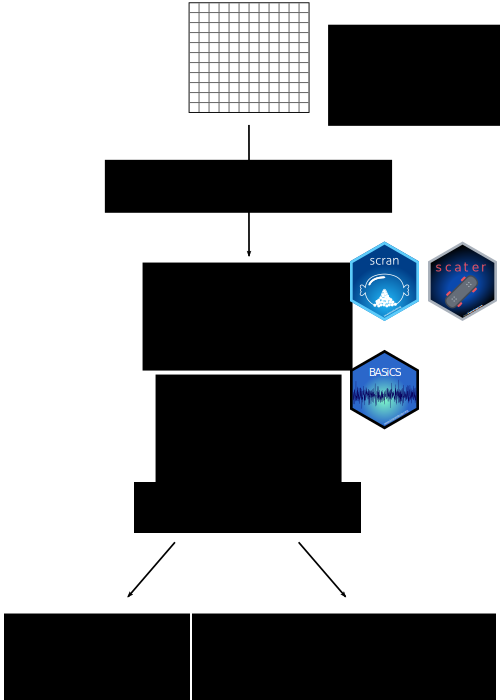
\includegraphics[width=2.5in,height=3.5in]{figure/Overview} 

}

\caption{Graphical overview for the scRNA-seq analysis workflow described in this manuscript. Starting from a matrix of expression counts, we use the scater and scran Bioconductor packages to perform QC and initial exploratory analyses. To robustly quantify transcriptional heterogeneity within seemingly homogeneous cell populations, we apply the BASiCS Bioconductor package and  illustrate how BASiCS can be used to analyse a single or multiple pre-specified groups of cells.}\label{fig:overview}
\end{figure}

\hypertarget{input-data}{%
\subsection{Input data}\label{input-data}}

\begin{Shaded}
\begin{Highlighting}[]
\KeywordTok{library}\NormalTok{(}\StringTok{"SingleCellExperiment"}\NormalTok{)}
\end{Highlighting}
\end{Shaded}

We use \emph{\href{https://bioconductor.org/packages/3.11/SingleCellExperiment}{SingleCellExperiment}} to convert an input
matrix of raw read-counts (molecule counts for UMI-based protocols) into a
\texttt{SingleCellExperiment} object which can also store its associated
metadata, such as gene- and cell-specific information.
Moreover, when available, the same object can also store read-counts for
spike-in molecules (see \texttt{altExp()}).
A major advantage of using a \texttt{SingleCellExperiment} object as the input for
scRNA-seq analyses is the interoperability across a large number of
Bioconductor packages \citep{Amezquita2019}.

\hypertarget{quality-control-and-exploratory-analysis}{%
\subsection{Quality control and exploratory analysis}\label{quality-control-and-exploratory-analysis}}

\begin{Shaded}
\begin{Highlighting}[]
\KeywordTok{library}\NormalTok{(}\StringTok{"scater"}\NormalTok{)}
\KeywordTok{library}\NormalTok{(}\StringTok{"scran"}\NormalTok{)}
\end{Highlighting}
\end{Shaded}

An critical step in scRNA-seq analyses is QC, removing low quality samples that
may distort downstream analyses.
Among others, QC diagnostics can help to identify samples that contain broken
cells, that are empty or that contain multiple cells \citep{Ilicic2016}.
Moreover, lowly expressed genes for which less reliable information is
available are typically also removed.
The \href{https://osca.bioconductor.org/}{\emph{OSCA}} online book provides an extensive
overview on important aspects of how to perform QC of scRNA-seq data, including
exploratory analyses \citep{Amezquita2019}.

Here, we use the \emph{\href{https://bioconductor.org/packages/3.11/scater}{scater}} package \citep{McCarthy2017} to calculate
QC metrics for each cell (e.g.~total read-count) and gene (e.g.~percentage of
zeroes across all cells), respectively.
Moreover, we use the visualisation tools implemented in \emph{\href{https://bioconductor.org/packages/3.11/scater}{scater}} to
explore the input dataset and its associated QC diagnostic metrics.
For further data exploration we use the \emph{\href{https://bioconductor.org/packages/3.11/scran}{scran}} package \citep{Lun2016}.
\emph{\href{https://bioconductor.org/packages/3.11/scran}{scran}} can perform \emph{global scaling} normalisation, calculating
cell-specific scaling factors that capture global differences in read-counts
across cells (e.g.~due to sequencing depth and PCR amplification)
\citep{Lun2016pooling}.
Moreover, \emph{\href{https://bioconductor.org/packages/3.11/scran}{scran}} enables exploratory analyses of transcriptional
variability.
For example, it can be used to infer an overall trend between mean expression
and the squared coefficent of variation (CV\textsuperscript{2}) for each gene.
To derive variability estimates that are not confounded by this overall trend,
\emph{\href{https://bioconductor.org/packages/3.11/scran}{scran}} also defines gene-specific DM (distance to the mean)
estimates as the distance between CV\(^2\) and a rolling median along the range
of mean expression values \citep{Kolodziejczyk2015cell}.
DM estimates enable exploratory analyses of cell-to-cell heterogeneity, but a
measure of uncertainty is not readily available. As such, gene-specific
downstream inference (e.g.~differential variability testing) is precluded.

\begin{Shaded}
\begin{Highlighting}[]
\KeywordTok{library}\NormalTok{(}\StringTok{"ggplot2"}\NormalTok{)}
\end{Highlighting}
\end{Shaded}

{\small\bibliography{Workflow.bib}}

\end{document}
